\documentclass[12pt]{thesis}

% The LaTeX default font is Computer Modern Roman for text and
% math. We will switch to times roman, because that is preferred by
% the Graduate school.  However, you can comment the times fonts and
% uncomment one (or more) of the others to choose a different font set.
\usepackage{mathptmx}   % Times New Roman with matching math fonts
% \usepackage{newcent}  % new century schoolbook font
% \usepackage{bookman}  % bookman font
% \usepackage{fourier}  % Utopia (text) and Fourier (math) font


\usepackage{graphicx}
\usepackage{rotating}
\usepackage{makeidx}
\usepackage{subfig}
\usepackage{indentfirst}

%% Uncomment the following two lines and comment out the third one
%% if you want to use the Chicago Manual based bibliography.
% \usepackage{thesiscitations}
% \bibliographystyle{thesis}
\bibliographystyle{ieeetr}

%% Change ieeetr in the previous line to any bibliography style you
%% like

%% Uncomment next line if you want chapter titles centered (not
%% approved by SDSMT graduate school)
% \centertitles

%% Uncomment next line to print a double-spaced draft version
% \dsdraft

%% Uncomment next line to print a single-spaced draft version
% \ssdraft

%% Uncomment next line if you are using makeindex to create an index
% \makeindex

\doctype{thesis}
\title{A Compative Study of Gnus and Gnats: The Most Important Paper Ever Written}
\author{Harvey Finklebaum}
\degree{Doctor of Philosophy in Zoology}
\defensedate{April 4, 2013}
\gradyear{2013}
\department{Zoology}

% The following commands add a signature line for each person who needs
% to sign the thesis/dissertation
\signatureline{Major Professor --- Dimm Whitt, Ph.D., Department of
  Zoology}

\signatureline{Graduate Division Representative --- E.\ Nigma, Ph.D.,
  Department of Philosophy}

\signatureline{Committee Member --- Chip Munk, Ph.D., Department of
  Zoology}

\signatureline{Committee Member --- Gail Force, Ph.D., Department of
  Meteorology }

\signatureline{Head of the Zoology Department --- Earl E. Byrd, Ph.D.}

\signatureline{Dean of Graduate Education --- Raney Daze}

\begin{document}

\maketitle

%% Comment the next line to remove the copyright notice.  Read the
%% section on copyright in the Thesis and Dissertation Writing
%% Instructions.
\makecopyright % copyright must go BEFORE \preliminaries


\preliminaries


\begin{abstract}
I present a fascinating and
thought provoking study, comparing gnus and gnats.
The results of the study show conclusively that there
is no resemblance between the two, whatsoever.
\end{abstract}

%% Uncomment the following if you want acknowledgements
\begin{acknowledgments}
  I would like to thank my advisor, Dr.\ Dimm Whitt, for
  all of the support he has given me. It really was not much,
  but he did at least stop yelling at me.
\end{acknowledgments}

\tableofcontents

\listoftables

\listoffigures

%% Uncomment following lines if you want a list of symbols
%% \gltitle{List of Symbols}
%% \begin{genericlist}
%% \begin{tabular}{ll}
%%   $\mathcal{G}_t$ & Gnat\\
%%   $\mathcal{G}_u$ & Gnu
%% \end{tabular}
%% \end{genericlist}

%% Uncomment following lines if you want a list of keywords
%% \gltitle{List of Keywords}
%% \begin{genericlist}
%% \noindent Gnat, Gnu
%% \end{genericlist}

%% Uncomment following lines if you want a dedication
% \begin{dedication}
% In loving memory of 
% my grandmother.
% \end{dedication}

%% Uncomment following lines if you want a preface
% \begin{preface}
% Before we begin, just let me say one thing.
% Gnat and gnu are both begin with ``gn,'' and
% the purpose of this work was to see if there
% are any other resemblances.
% This thesis has taken 45 years of work, and
% I don't have much time left in this world, but it
% has been worth it.  When the time comes,
% I would like to die as my grandmother did, peacefully in
% her sleep, not screaming like the passengers in her car.
% \end{preface}


\body


\chapter{Introduction}
This thesis is the first work ever done in 
the fascinating study of comparison of gnats to gnus.
It is groundbreaking.  There literally is nothing
like it.   However, there have been a few studies
of other things.

\chapter{Previous Work}


There has been a lot of previous work that is not at all like my work.
For example,
% The following if-then-else allows us to get good results with
% any bibliography/citation style.
\ifthesiscitations
\citeN{Kringle} % if we are using the thesiscitations style
\else
Kringle~\cite{Kringle} % if we are using a more primitive citation style
\fi
showed that apples and goats have almost
nothing in common, other than both being red.  The major problem with
Kringle's study is that he used a goat that had been spray painted
red, and his apple was a golden delicious variety.  Criticism of
Kringle's methods has been harsh, and so far, no one has been able to
replicate his results.

Several researchers have compared trout to
eagles~\cite{Simmons,Sheppard}.  The consensus that has emerged is
that they are quite different, and only an idiot would try to eat an
eagle~\cite{Idiot}.

\chapter{Methods}
In this chapter, I will present the methods for my comparison, and
fill in with a lot of gibberish.  For instance, I will say things like
``Gnats and Gnus come in twos'' in order to fill space and make my
thesis seem longer than it really is.  This is a tactic used by some
people to hide the fact that their research is worthless.  The idea is
that if the thesis is long enough and boring enough, the thesis
comittee members will go to sleep every time they try to read it.

Another thing that I may do is to use very long words, such as
onomatopoeia, for no apparent reason.  By employing voluminous
instances of obfuscatory and expansive vocables, the lack of
quintessence of this monograph can be adumbrated from all but
the most erudite, didactic, and scholarly bibliophiles.


\chapter{Results}
My research had fabulous results. I will now tell you about
the results, because they are the best!  You are not going
to believe how good my results are.

\section{Visual comparison}
%\index{comparison!visual}

\begin{table}
\caption{Results of visual comparison studies.}
\begin{center}
  \begin{tabular}{|c|c|}
    \hline
    \bf Categories & \bf Percent Correct\\
    \hline
    \hline
    insect/mammal & 76\\
    \hline
    gnat/gnu & 69\\
    \hline
  \end{tabular}
\end{center}
\label{table:comp1}
\end{table}

The first test that I performed was a visual comparison of gnats and
gnus.  First, I went on the internet and downloaded several thousand
pictures of gnats, and one picture of a gnu.  Then, I had two
volunteers compare them and categorize them as insect
%\index{insect}
or mammal.
%\index{mammal}
Next, I selected another group of volunteers and
had them classify the photographs as either gnat or gnu.


\begin{sidewaysfigure}
\begin{center}
\subfloat{\resizebox{0.45\textheight}{!}{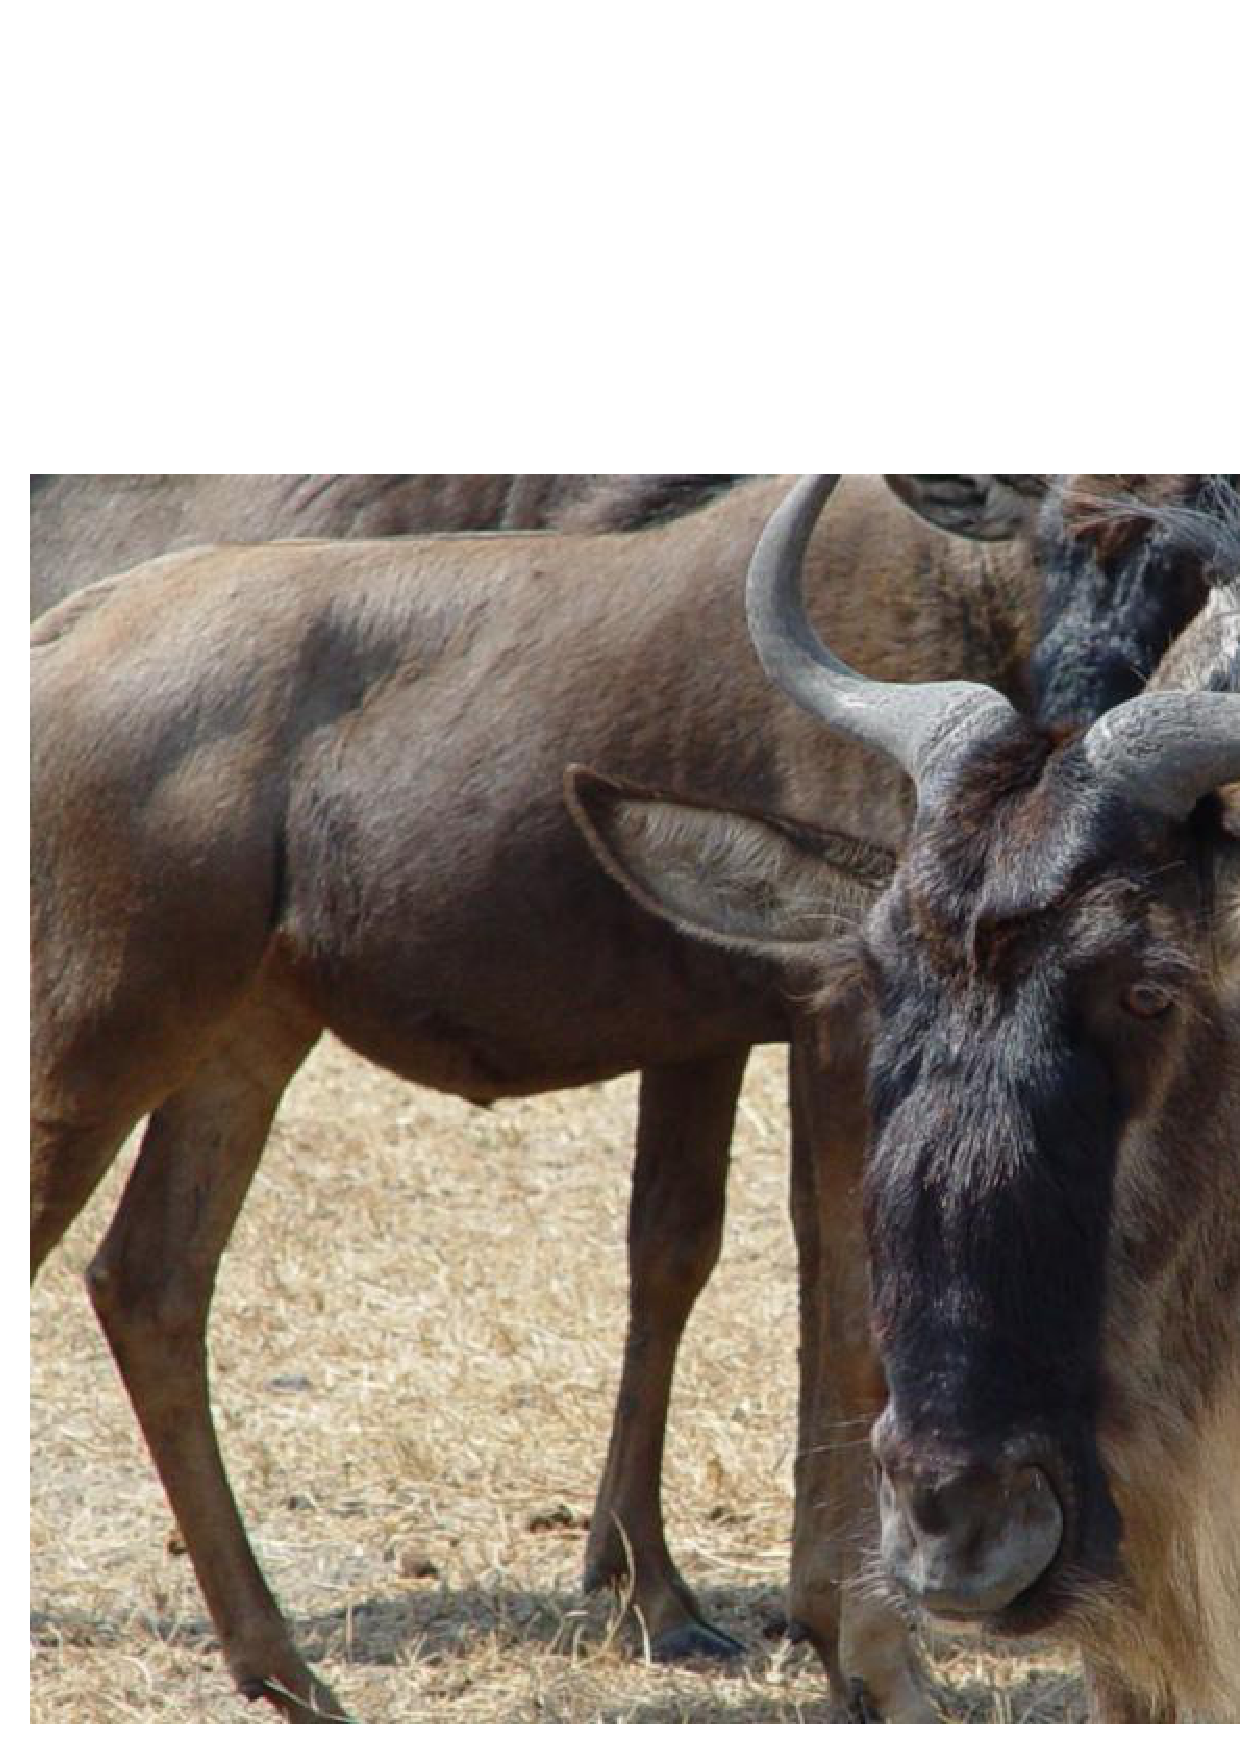
\includegraphics{images/gnu.pdf}}}
\subfloat{\resizebox{0.45\textheight}{!}{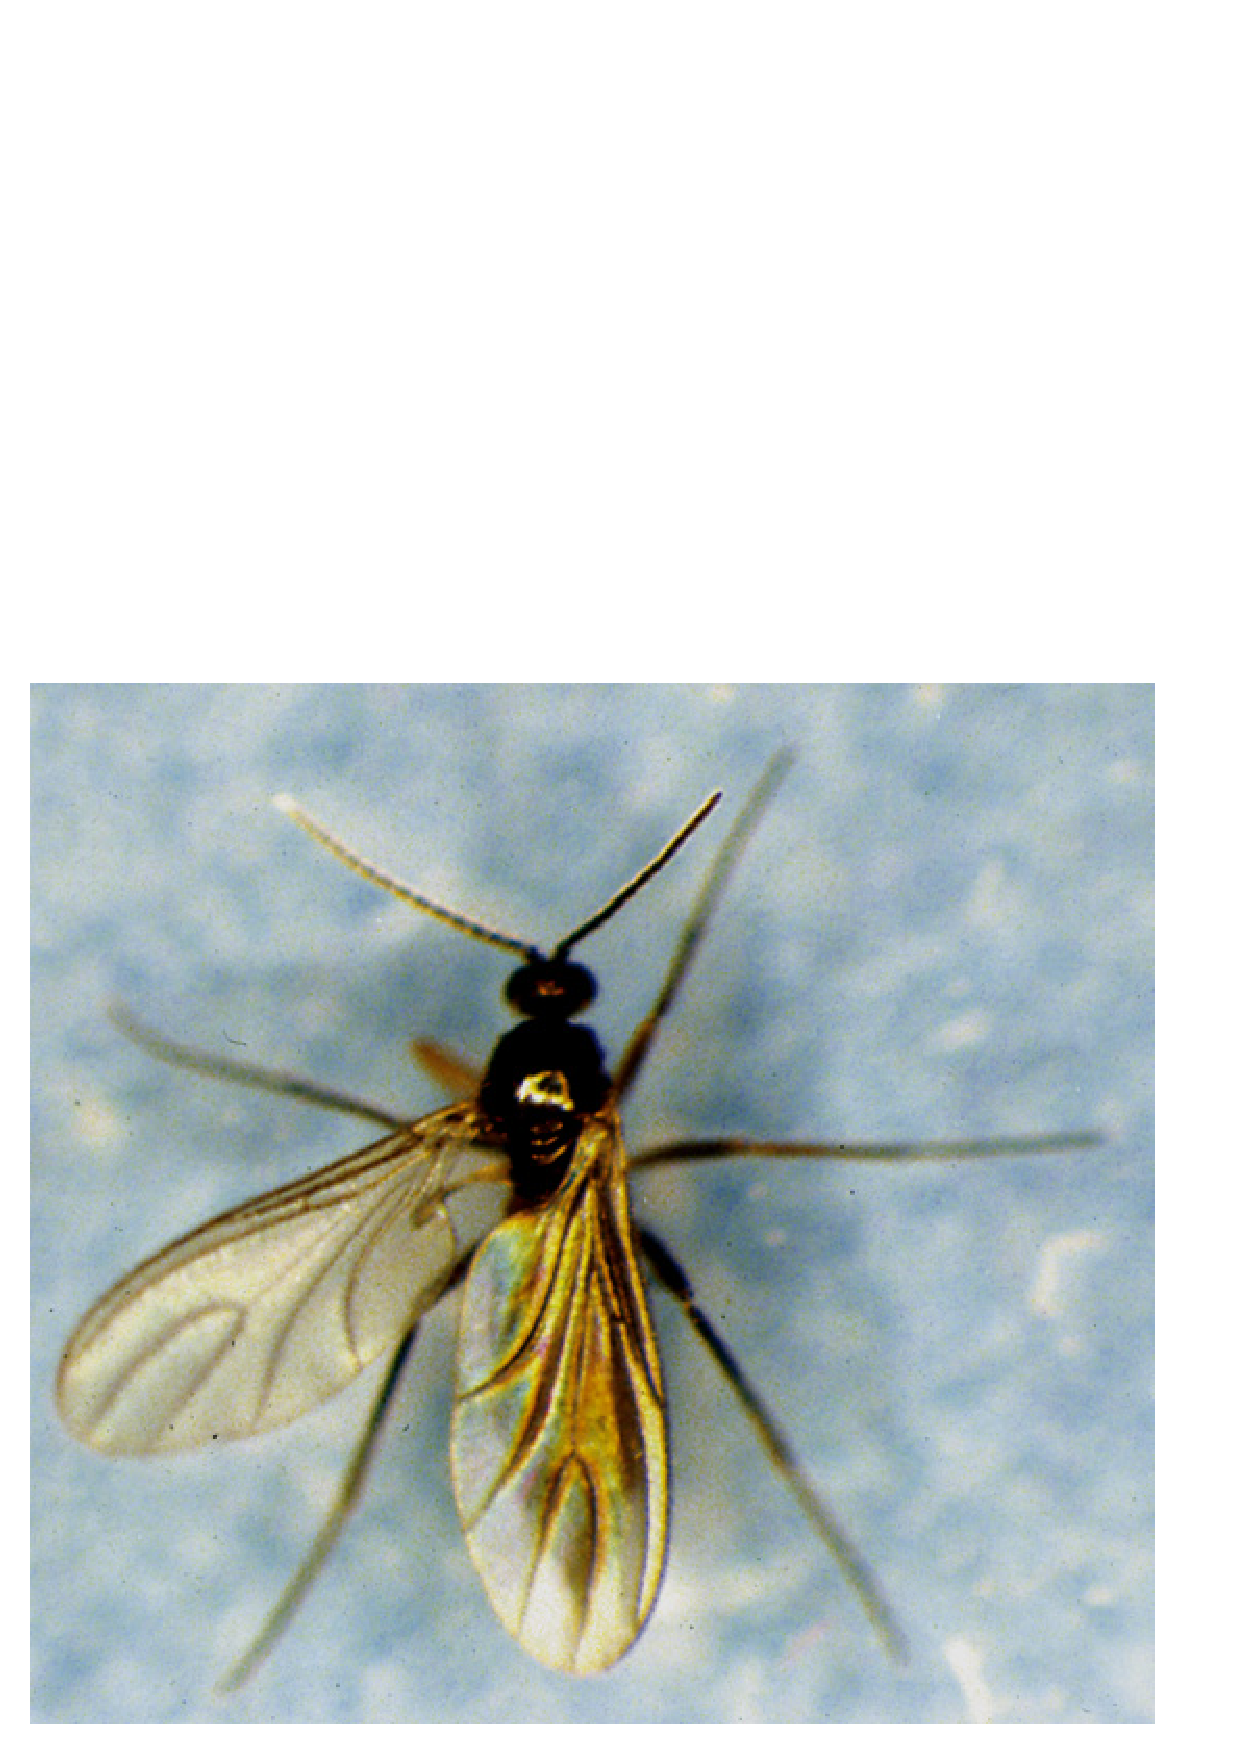
\includegraphics{images/gnat.pdf}}}
\end{center}
\caption{Photographs of a gnu (left) and a gnat (right).}
\label{figure:photos}
\end{sidewaysfigure}

The results of this comparison are shown in Table~\ref{table:comp1}.
As can be seen, both volunteers (myself and my advisor) were able to
correctly classify most of the photographs.  As a result, we gave each
other little gold stars.
For those who are interested, Figure~\ref{figure:photos} shows the gnu
photograph and one of the gnat photographs.

\section{Comparison by Size}
\index{comparison!size} As can be seen from
Figure~\ref{figure:photos}, photographs of gnats are slightly larger
than photographs of gnus.  This leads us to believe that
statistically, gnats are slightly larger than gnus.  Mathematically,
we express this as follows:
\begin{equation}
S(\mathcal{G}_t) > S(\mathcal{G}_u) \forall
\mathcal{G}_t,\mathcal{G}_u,
\end{equation}
where $\mathcal{G}_t$ is a photograph of a gnat and $\mathcal{G}_u$ is
a photograph of a gnu.  The $S()$ function calculates the ``size'' of
the photograph.

\chapter{Conclusions}

Well, there you have it.  My advisor and I were able to tell the
difference between a photograph of a gnat and a gnu most of the time.
Also, gnats are larger than gnus, and therefore, they are
significantly different.

In the future, we plan to apply the techniques developed in this
research to answer the age old question of whether dogs and ducks are
the same thing.

\supplementaries


\bibliography{harvey}


\begin{appendices}

\appendix{Appendix A} Well, I really have nothing more to say,
but wanted to have an appendix.

\end{appendices}

%% Uncomment the following lines if you want to create a glossary
% \begin{gloss}
% I don't have a glossary either, but this is what the page would look
% like if I did.
% \end{gloss}


%% uncomment following lines if you want to create a list of abbreviations
% \begin{abbreviations}
% gnu is abbreviated to gnu\\
% gnat is abbreviated to gnat
% \end{abbreviations}

%% uncomment next line if you used makeindex to make an index
%\printindex

\begin{vita}

  
  Format the vita page according to the following graduate school requirements:

A vita page, not over one page in length, is to be included as the
last page of all theses and dissertations deposited in the Devereaux
Library. The vita is to be written in the third person using
professional style and could contain the following information
(although you may wish to omit A and B if concerned about identity
theft):
\begin{enumerate}[label=\Alph*.]
\item Place and date of birth.

\item Place and date of high school graduation.

\item Place and date of college graduation—with degree and major.

\item Place and date of receipt of master’s degree—with major.

\item Vocational and professional experience (not summer jobs)—including dates, nature of position, and school or organization.

\item Military experience, with indication of professional relevance—if any.

\item Scholarly publications, exhibits of creative work, membership in professional organizations and honorary societies.
\end{enumerate}
  

\end{vita}



\end{document}
